\documentclass[a4paper,11pt]{article}

\usepackage[T1]{fontenc}

\usepackage[utf8]{inputenc}

\usepackage[italian]{babel}

\usepackage{graphicx}

\usepackage{indentfirst}

\usepackage{amsmath,amssymb}

\usepackage{enumitem} 

\newcommand{\virgolette}[1]{``#1''}

\usepackage[margin=1in]{geometry} %Smaller margins

\usepackage{lmodern} %Vector PDF

\usepackage{siunitx}

\usepackage{xcolor}

\usepackage{colortbl}

\usepackage{multirow}

\usepackage{rotating}

\usepackage{booktabs}

\usepackage{longtable}

\usepackage{graphicx}
\graphicspath{ {../../Immagini/} }

\usepackage{wrapfig}

\usepackage{siunitx} % Per unità di misura in generale e la corretta rappresentazione dei numeri.

\usepackage{gensymb} % Per il simbolo di gradi


\begin{document}
	\section{Strumentazione} \label{strum}
\begin{wrapfigure}{R}{0.5\textwidth}
	\caption{Schema interferometro}\label{interf}
	\centering
	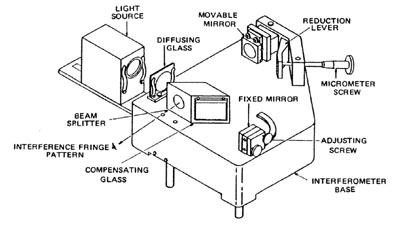
\includegraphics[width=0.48\textwidth]{interf}
\end{wrapfigure}
Poiché l'esperimento aveva più obiettivi la strumentazione ha coinvolto componenti diverse a seconda della misura che si stava effettuando. Ci sono stati però degli strumenti indispensabili per tutta l'esperienza. In generale però la strumentazione usata era composta da:
\begin{description}
	
	\item[Interferometro di Michelson] Questo è stato il principale e più importante strumento utilizzato. L'interferometro è stato utilizzato per creare figure di interferenza in modo controllato. La figura \ref{interf} rappresenta schematicamente un interferometro simile a quello usato nel laboratorio.\\
	È utile per la spiegazione delle componenti dell'interferometro descrivere il suo funzionamento. Dopo essere usciti dalla sorgente (\virgolette{light source}) i raggi di luce entravano un dispositivo a forma di prisma con i lati di vetro che aveva il compito di dividere in due il fascio di luce (\virgolette{beam splitter}).
	Questo era fisso alla base dell'interferometro (\virgolette{interferometer base}) ed era trasparente sui lati, per permettere il passaggio della luce. Al suo interno era presente uno specchio semiriflettente (con la parte riflettente posta verso l'interno), e tre vetri piani. Lo specchio semiriflettente e il vetro opposto ad esso erano angolati di $ 45\degree $ rispetto agli altri due. Mentre i due vetri opposti l'uno all'altro non avevano una funzione vera e propria, il vetro opposto allo specchio semiriflettente (\virgolette{compensating glass}) serviva per ovviare le differenze dei percorsi dei due raggi spezzati.\\
	Dopo essere stati divisi dal dispositivo sopra i raggi di luce procedevano per due strade diverse. Uno procedeva in avanti, verso uno specchio fisso (\virgolette{fixed mirror}). Questo era regolato in fase di calibrazione e lasciato fermo. Per la calibrazione erano presenti due viti (\virgolette{adjusting scew}) una che regolava la sua angolazione rispetto alla base dell'interferometro ed una che regolava la sua angolazione rispetto allo specchio mobile. Quindi, dopo essere stato riflesso dallo specchio fisso il vetro tornava indietro verso il \virgolette{beam splitter}. Il secondo raggio di luce invece procedeva verso lo specchio mobile (\virgolette{movable mirror}). La sua angolazione rispetto alla base dell'interferometro non era regolabile, quindi si può supporre che sia perfettamente perpendicolare. La posizione dello specchio mobile era regolabile attraverso una vite micrometrica (\virgolette{micrometer screw}). La precisione di questa era ulteriormente aumentata di un fattore cinque da un sistema di leve (\virgolette{reduction lever}). Quindi dopo essere riflesso dallo specchio mobile il raggio ritornava verso il \virgolette{beam splitter}.\\
	Una volta riincontrati i raggi erano quindi riflessi verso lo schermo (non rappresentato in figura) dove formavano una figura di interferenza.

\end{description}

\begin{description}
	
	\item[Laser] Era presente uno strumento che generava un raggio laser. Il funzionamento di questo strumento va oltre gli scopi dell'esperienza. Sul dispositivo erano presenti delle informazioni scritte dal costruttore, secondo cui il raggio generato sarebbe stato di $ 633\si{\nano\meter} $.
	\item[Lente] Per rendere il fascio di luce laser più visibile è stata usata una lente convergente con distanza focale molto piccola. La lente permetteva di allargare il fascio luminoso per distinguere meglio le frange di interferenza.
	\item[Cameretta per il vuoto] Per la misura dell'indice di rifrazione dell'aria è stato usata una cameretta per il vuoto. Questa è stata fissata tra il \virgolette{beam splitter} e lo specchio fisso e aveva due lati trasparenti per permettere il passaggio della luce. La camera interna (lunga $ \SI{5}{\centi\meter}$) era collegata tramite un sistema di valvole e tubi ad una pompa per il vuoto che permetteva di creare il vuoto e lentamente far rientrare l'aria.
	\item[Una lampada al sodio] Usata per misurare la differenza di lunghezza d'onda tra le due lunghezze più visibili.
	\item[Una sorgente di luce bianca] Usata per misurare le dimensioni dei pacchetti d'onda.
	\item[Schermo] Le figure di interferenza erano proiettate su uno schermo bianco. Erano a disposizione due schermi, uno retto da un piccolo piedistallo sul tavolo di lavoro e uno appeso al muro di fronte (a circa $ \SI{3}{\meter} $ dall'interferometro).
\end{description}

\end{document}
